\documentclass[a4paper]{article}
%% Language and font encodings
\usepackage[T1]{fontenc}

%% Useful packages
\usepackage{amsmath}
\usepackage{pbox}
\usepackage{float}
\usepackage{indentfirst}
\usepackage{graphicx}
\usepackage[colorinlistoftodos]{todonotes}
\usepackage[colorlinks=true, allcolors=blue]{hyperref}

\usepackage[utf8]{inputenc} % allow utf-8 input
\usepackage{hyperref}       % hyperlinks
\usepackage{url}            % simple URL typesetting
\usepackage{booktabs}       % professional-quality tables
\usepackage{amsfonts}       % blackboard math symbols
\usepackage{amsmath}
\usepackage{amsthm}
\usepackage{amssymb}
\usepackage{bm}
\usepackage{nicefrac}       % compact symbols for 1/2, etc.
\usepackage{microtype}      % microtypography
\usepackage{listings}		% to embed R code later
\usepackage{graphicx}		% to embed images later
\graphicspath{ {images/} }	% to embed images later

\usepackage{tabularx,ragged2e,booktabs,caption}
\newcolumntype{C}[1]{>{\Centering}m{#1}}
\renewcommand\tabularxcolumn[1]{C{#1}}

\title{Case Study 3: Final Report}
\author{Steve Kang, Sam Yin, Aibi Janat}

\begin{document}
\maketitle

\begin{abstract}
In this report, we examined length of survival and gene expressions for 240 subjects. In order to reduce number of covariates from 7,399 to 500, we first conducted independent screening using Cox model. Afterwards, we imputed censored data using an algorithm similar to Markov Chain Monte Carlo. As for variable selection and prediction, we used Weighted Latent Factor Regression as well as LASSO model. The result indicates that Weighted Latent Factor Regression ($w$ = 0.1) has the best overall performance, especially when trained with the uncensored data.
\end{abstract}

\section{Model Introduction}

\subsection{Independent Screening}
The data set has an extremely large number of 7,399 covariates so we conducted independent screening to reduce number of covariates down to 500 variables using only the uncensored observations. We used Cox model, a statistical technique that is used for exploring the relationship between the survival of a patient and several explanatory variables. It allows estimation of the hazard of death for individuals, given their prognostic variables such as gene expressions. Using the hazard model below where $X_{i}$ represents the realized values of the covariates for subject i, we computed p-values for each covariate coefficient:
$$\lambda(t|X_{i}) = \lambda_{0}(t)\exp(\beta X_{i})$$

We decided to keep 500 variables with the lowest p-values ranging from 2.15E-06 to 1.03E-0.2 after trial and error with the imputation process discussed below, because keeping too few variables resulted in many imputed values not converging. Below shows a histogram of p-values for all 7,399 gene expressions.

\begin{figure}[H]
\centering
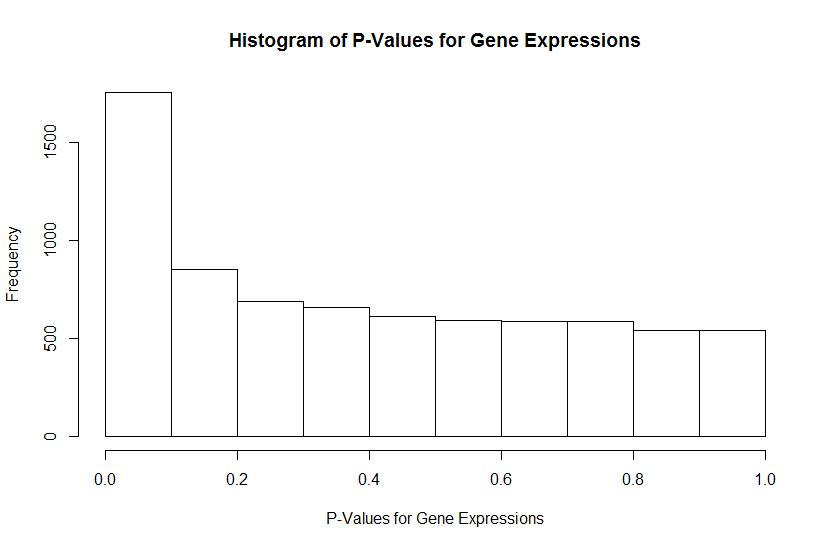
\includegraphics[width=60mm]{pvalue.png}
\caption{Histogram of P-values from Independent Screening}
\end{figure}

\subsection{Imputation}
The imputation in this analysis assumes that there is no systematic difference between censored observations and uncensored ones, which implies that they came from the same distribution and can be described by the same model (see further examination of whether the censored data differ significantly from the uncensored in modeling section). If this assumption holds, data imputation adopts a multivariate regression model for survival time of all patients (with log transformation): $$\log(y_{i}) = \alpha + {\theta}^{T}\mathbf{x}_{i} + \epsilon_{i}$$ where $(\mathbf{x}_{i}, y_{i})$ is an observation from the data set, $\alpha$ is the baseline level of survival time (with log transformation) in absence of any effect of gene expression level, ${\theta}$ is a vector of coefficients for covariates, $\epsilon_{i} \sim N(0, \sigma)$ denotes the error.

The algorithm of data imputation is as follows: 
\begin{enumerate}
\item set $\theta^{(0)}$, $\sigma^{(0)}$, and $y_{j}^{(0)} \text{ for }j = 1, 2, \ldots, N_{\text{censored}}$
\item for $t = 1, 2, \ldots, T$
\begin{enumerate}
\item $\log(y_{j}^{(t)}) \sim \textrm{Truncated Normal}(\alpha + \mathbf{x}_{j}^{T}\theta^{(t - 1)}, \sigma^{(t - 1)}; L = \log(y_{j}^{(0)})) \,$
\item update $\theta^{(t)}$ and $\sigma^{(t)}$ with all uncensored and imputed data in the current step
\end{enumerate}
\end{enumerate}

Notice that the structure of the algorithm above is similar to Markov Chain Monte Carlo, thus the code was implemented in RStudio with Stan package (1 chain, 2,000 iterations). The lower bound of the truncated normal distribution where $y_{j}^{(t)}$ was sampled from is equal to the survival time collected in the original data set, for the subject must have had survived longer than that time period. The sampler only vastly explored the hypothesis space when moderate noise was introduced to the initial value of $y_{j}$'s and when the standard deviation was relatively significant.

Most imputed survival time reached convergence (Rhat, scale reduction factor on split chains, close to 1) with a few exceptions. Therefore, the sampling means (the algorithm was repeated 20 times and the mean corresponding to the lowest Rhat was selected) were used as estimates of right-censored data points and merged with the uncensored data for analysis.

\subsection{Variable Selection and Predictive Modeling: LASSO and Weighted Latent Factor Regression}
In general, a specific symptom or disease is associated with only a small number of genes. Therefore, among all the genes present in the data set, we can assume that only a small proportion are directly linked to lymphoma. In other words, if we apply regression analysis, the coefficient matrix between gene predictors and survival time will be rather sparse, of which most entries are (close to) zero. Considering this important feature of data structure, we apply $l1$-norm regularized regression or LASSO (least absolute shrinkage and selection operator), which controls for sparsity and tends to select one variable out of a highly-correlated pair/group, as a primary candidate for modeling approach. In contrast to non-regularized linear regression model, the estimate of coefficient parameter $\bm{\beta}$ for LASSO is $$\hat{\bm{\beta}} = \arg\min_{\bm{\beta} \in \mathbb{R}^{p}}\|y - \mathbf{X}^{T}\bm{\beta}\|_{2}^{2} + \lambda\|\bm{\beta}\|_{1} (\lambda > 0).$$

The large number of available explanatory variables in the data set for survival time implies a high level of multicollinearity and complex interaction among genes. An alternative modeling method is to assume that several groups of certain genes tend to form pathways and collectively facilitate (or undermine) the survival of subjects. These pathways can be modeled as $k$ latent factors ($k << p$, where $p$ is the number of variables in the original data set), given which the predictors and the response are conditionally independent (from the perspective of graphical models). This latent factor model could be formulated as follows:
$$\mathbf{X}_{i} \sim \bm{\eta}_{i}\bm{\lambda}^{T} + \bm{\epsilon}$$
$$\mathbf{Y}_{i} \sim \bm{\eta}_{i}\bm{\theta} + \bm{\varepsilon}_{i}$$
where $\bm{\eta}$ is an $n \times k$ matrix where the $i^{\text{th}}$ row includes the level of all latent factors for subject $i$, $\bm{\lambda}$, the factor loading matrix, is an $p \times k$ matrix where the $h^{\text{th}}$ column indicates the weight of all gene predictors in the $h^{\text{th}}$ latent factor, $\bm{\theta}$ is a vector of length $k$ with coefficients of latent factors in the linear regression model for survival time $\mathbf{Y}$, and $\bm{\epsilon}_{j} \sim N(0, \sigma_{j})$, $\bm{\varepsilon}_{i} \sim N(0, \sigma_{y})$ represent the error.

A pressing problem with the usual likelihood formulation is that for each subject, the contribution to the likelihood from gene predictors outweighs that from survival time to a great extent (in this analysis, the product of 500 Gaussian likelihood versus one). As a result, the latent factors will capture primarily the characteristics of explanatory variables but relatively minimal information of survival time, which significantly affects the predictive power. An explicit correction is to down-weight the likelihood of gene predictors by multiplying it with a coefficient $w (0 < w < 1)$ in the log likelihood function: $$\log \mathcal{L}(\mathbf{X}, \mathbf{Y}|-) = \sum_{i = 1}^{n}[w\sum_{j = 1}^{p}\log(Normal(\mathbf{x}_{i, j}; \bm{\eta}_{i}\bm{\lambda}^{T}, \bm{\epsilon})) + \log(logNormal(y_{i}; \bm{\eta}_{i}\bm{\theta}, \varepsilon))].$$ If the magnitude of weight parameter $w$ is close to 0, the prediction tends to be centralized so that the variance of survival time cannot be captured precisely. In contrary, if $w$ is close to 1, some of the predictive values exceed the normal range of survival time. The value of $w$ was set as 0.1, 0.25, 0.5, and 1 in this analysis for comparison.

Since most of the genes only belong to a few pathways and most of the pathways involve a small number of genes, a majority of the entries in $\bm{\lambda}$ are close to 0. In order to control for sparsity and to impose varying levels of shrinkage among latent factors, the following prior (based upon Bhattacharya \& Dunson, 2011) was applied in sampling: 
$$\lambda_{jh}|\phi_{ih}, \tau_{h} \sim N(0, \phi_{ih}^{-1}\tau_{h}^{-1}), \phi_{jh} \sim Ga(\nu/2, \nu/2), \tau_{h} = \prod_{l = 1}^{h}\delta_{l}$$
$$\delta_{1} \sim Ga(a_{1}, 1), \delta_{l} \sim Ga(a_{2}, 1), l \geq 2, \sigma_{j}^{-2} \sim Ga(a_{\sigma}, b_{\sigma}), \sigma_{y}^{-2} \sim Ga(a_{y}, b_{y}),$$ where the variance of $\lambda_{jh}$ is composed of local ($\phi_{jh}$) and global/factor-wise ($\tau_{h}$, with increasing precision as column index increases) parameters.

Both of the models are trained on $3/4$ of the data set (both for uncensored data set only and the entire data set with imputed values) and tested on the other $1/4$. The factor loading matrices and regression coefficient parameters after training were used in generating prediction of survival time in the test set. The models are trained on RStan platform, and the parameter estimates are sampling means (1 chain, 500 iterations). The performance is measured by root mean squared error as $\sqrt{\frac{1}{n}\sum_{i = 1}^{n}(\hat{y}_{i} - y_{i})^{2}}$.

\section{Result Interpretation \& Model Fitness}

\begin{center}
\begin{minipage}{\linewidth}
\centering
\captionof{table}{Model Trained with the Combined Data} \label{tab:title}
\begin{tabular}{|c|c|c|c|}
\hline	
Model & RMSE & Parameters \\
\hline\hline
Weighted Latent Factor ($w$=0.1) & 38.007 & 0 lambda coefficients (>0.05) \\
\hline
Weighted Latent Factor ($w$=0.25) & 38.316 & 234 lambda coefficients (>0.05) \\
\hline
Weighted Latent Factor ($w$=0.5) & 38.065 & 164 lambda coefficients (>0.05) \\
\hline
Weighted Latent Factor ($w$=1) & 38.022 & 151 lambda coefficients (>0.05) \\
\hline

LASSO & 39.325 & 173 non-zero coefficients \\
\hline
\end{tabular}
\end{minipage}
\end{center}

When the five models (four Weighted Latent Factor Models and LASSO Model) are trained with the combined data, the Weighted Latent Factor Model with $w$ = 0.1 performs the best in terms of RMSE (38.007). However, none of the lambda coefficients is larger than 0.05, leading to very low variance in predicted values (all predicted values hovered around 4.0). When $w$ is larger, there are more significant lambda coefficients. This means that when $w$ is small, latent vectors become more sparse because predictors contribute less to the likelihood function.

On the other hand, the Unweighted Latent Factor Model ($w$ = 1) had the highest percentage of accurately predicting survival time (margin of error = 3). It accurately predicted 62$\%$ of the time whereas the other models accurately predicted 52$\%$, 50$\%$, 55$\%$, and 47$\%$ of the time, respectively. This shows that when $w$ is high, more variance is introduced to the model for more accurate prediction. When $w$ is too small, the model is not really predicting using the information from gene expressions. The performance of the two models ($w$ = 0.1 and $w$ = 1) in prediction can be found below:

\begin{figure}[H]
\centering
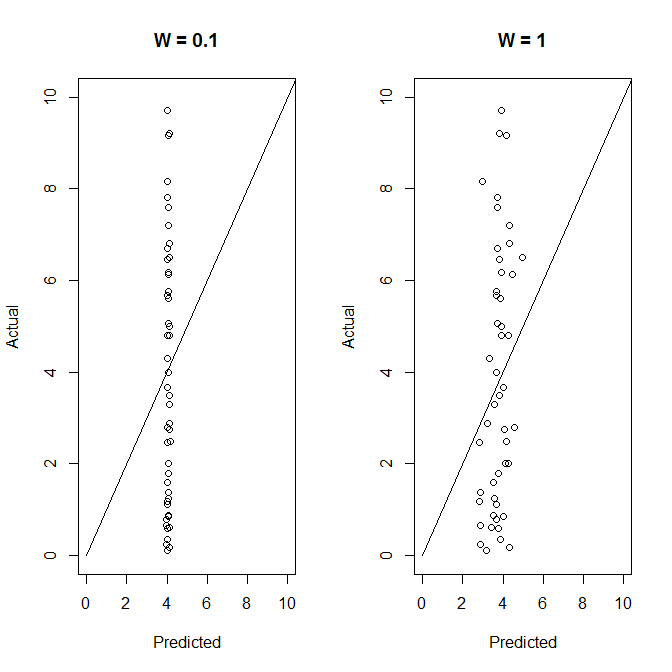
\includegraphics[width=80mm]{W_comparison.png}
\caption{Predicted vs. Actual Plots for $w$ = 0.1 and $w$ = 1 Models}
\end{figure}

\begin{center}
\begin{minipage}{\linewidth}
\centering
\captionof{table}{Model Trained with the Uncensored Data} \label{tab:title}
\begin{tabular}{|c|c|c|c|}
\hline	
Model & RMSE & Parameters \\
\hline\hline
Weighted Latent Factor ($w$=0.1) & 3.190
 & 42 lambda coefficients (>0.05) \\
\hline
Weighted Latent Factor ($w$=0.25) & 5.265
 & 148 lambda coefficients (>0.05) \\
\hline
Weighted Latent Factor ($w$=0.5) & 3.776
 & 815 lambda coefficients (>0.05) \\
\hline
Weighted Latent Factor ($w$=1) & 7.331e+81
 & 8,940 lambda coefficients (>0.05) \\
\hline
G-LASSO & 4.797 & 85 non-zero coefficients \\
\hline
\end{tabular}
\end{minipage}
\end{center}

Similarly, when the five models are trained with the uncensored data, the Weighted Latent Factor Model with $w$ = 0.1 performs best in terms of RMSE (3.190). This model only has 42 significant lambda coefficients with values larger than 0.05 whereas the other models with higher $w$ have more lambda coefficients with such values.

In addition to having the lowest RMSE value, the Weighted Latent Factor Model (w = 0.1) has the second highest percentage (52$\%$) of accurately predicting survival time (margin of error = 3) while the model with $w$ = 0.25 has the highest percentage (56$\%$). The other models accurately predict 48$\%$, 4$\%$ and 28$\%$ of the time, respectively.

The performance of the two models ($w$ = 0.1 and $w$ = 0.25) in prediction can be found below and we can see that more variance is introduced to the model with higher $w$ value:

\begin{figure}[H]
\centering
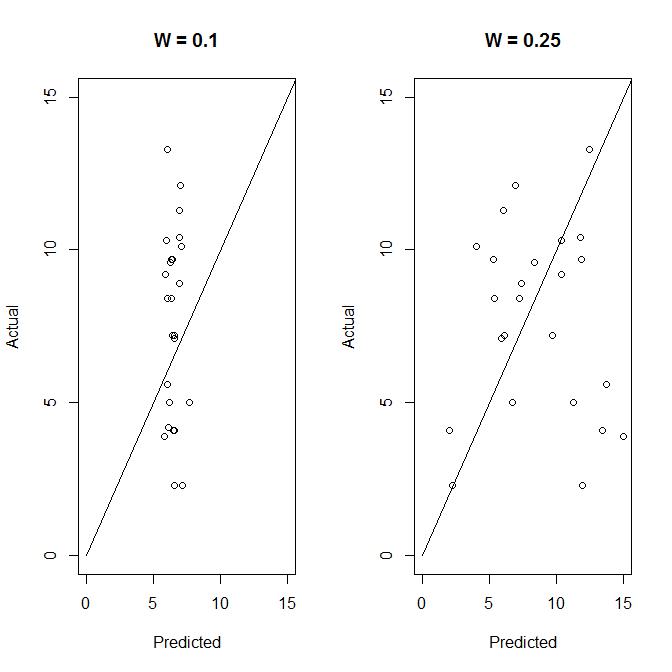
\includegraphics[width=80mm]{pred_uncens.png}
\caption{Predicted vs. Actual Plots for $w$ = 0.1 and $w$ = 0.25 Models}
\end{figure}

When significant coefficients of the Weighted Latent Factor ($w$ = 0.1) and LASSO models trained with the uncensored data are compared, there are several overlapping gene expressions including Gene 2044, 3251, 3812, 4127, 6508 and 6897. To understand the biological significance of these gene expressions, it would be important to locate them in the genome and then decide whether including interaction terms between some of these genes and others would be valid.

When comparing the results of the models trained with the combined data versus uncensored data, we can tell from much smaller RMSE values that the model trained with the uncensored data always does better. This is likely the case because some imputed survival time values are beyond the normal range, leading to extremely large error terms in prediction.

For both training scenarios, there are still large numbers of "unique" significant predictors (counting variables only once if they were significant in more than 1 latent factor) with respect to the number of observations, which suggests the potential risk of model overfitting.

On the other hand, LASSO regularizes the $l1$-norm, thus yielding a sparse vector of coefficients in the model after training, with 327/415 out of 500 predictors with no influence on the survival time. Among the variables with nonzero effect, the coefficients are between -0.4 and 1.3 for the combined data set and between -0.2 and 1.9 for the uncensored data set (with standardization). The performance in prediction is much better if LASSO is trained with the combined data set, because the censored data is imputed under the assumption of a linear relationship. Also, there are more significant predictors in the model trained on the combined data set (173 for the combined data set vs. 85 for the uncensored data set). Nonetheless, there is a large number of significant predictors with respect to the number of observations, which implies again the potential risk of model overfitting. In terms of variable selection, LASSO just picks one variable from each group of highly correlated ones to include and excludes the rest. In order to determine which genes are predictive, it will be necessary to identify variables from LASSO that were found to be important with non-zero coefficients and then examine covariates that were highly correlated with these variables.

\section{Further Discussion}

For the Latent Factor Model, we could enhance the model by experimenting with a different number of latent variables to compare model performance. Alternatively, an adaptive process of choosing the number of latent factors could be adopted. The challenge lies in the model's low computational efficiency due to the large number of parameters in the model. Model simplification or significant change to algorithm is required to increase computational speed.

One way we could improve both models is to explore potential interaction terms between covariates. Certain pairs or groups of genes may work together in affecting the survival time. In order to incorporate these terms to the current models, we need to have prior information on genes and a valid metric for auto-correlation to facilitate selection of interaction terms. Moreover, the risk of model overfitting and under-identification becomes more salient as the number of variables increases.

In addition, we could explore different values of the weight parameter by grid search with cross validation and strike a balance between the predictive power and variation of estimates. Also, we could explore down-weighting the imputed survival time values compared to the uncensored values to ensure that the more accurate values are weighted more in the model.

\section*{Role of Authors}

Steve: Independent Screening, Variable Selection, Write-up

Sam: Imputation, Modeling and Evaluation, Write-up

Aibi: Variable Selection, Write-up

\section*{Reference}
Bhattacharya, A., \& Dunson, D. B. (2011). Sparse Bayesian infinite factor models. Biometrika, 98(2), 291-306.

\end{document}